\documentclass[dvipdfmx,autodetect-engine,titlepage]{jsarticle}
\usepackage[dvipdfm]{graphicx}
\usepackage{ascmac}
\usepackage{fancybox}
\usepackage{listings}
\usepackage{plistings}
\usepackage{itembkbx}
\usepackage{amsmath}
\usepackage{svg}
\usepackage{url}
\usepackage{graphics}
\usepackage{listings,jvlisting}

\textheight=23cm
\renewcommand{\figurename}{図}
\renewcommand{\tablename}{表}
\newenvironment{code}
{\vspace{0.5zw}\VerbatimEnvironment  \begin{screen} 
\baselineskip=1.0\normalbaselineskip
 \begin{Verbatim}}
{\end{Verbatim}
\baselineskip=\normalbaselineskip
 \end{screen}\vspace{0.5zw}} 

\title{情報理工学部 SNコース 2回\\
セキュリティ・ネットワーク学実験2\\
課題4-4レポート}
\author{2600200443-6\\Yamashita Kyohei\\山下 恭平}
\date{Oct 17 2021}

\begin{document}

\maketitle

\section{概要}
Android StudioとAndroidのエミュレーターを用いて、Android端末に搭載されているセンサから取得した情報を、
端末上に表示するプログラムの開発、および、取得した情報をリアルタイムでグラフとして画面上に表示するアプリケーションの開発。

\section{外部仕様}

 \subsection{開発対象の使い方に関する説明}

 この実験ではアンドロイドスマートフォンをエミュレーターを用いて利用している。\\
 主に使用する機能は、ディスプレイおよび地磁気センサである。地磁気センサの値は
 エミュレーターの設定により自由に設定することが可能である。
 
 \begin{figure}[h]
    \centering
    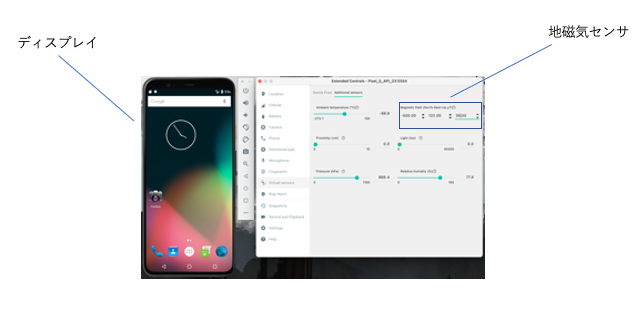
\includegraphics[scale=0.4]{pic0.png}
  \end{figure}
 
 \subsection{開発対象を構成するハードウェアと、その主な仕様}

 今回主に使用したハードウェアは地磁気センサである。\\
 地磁気センサはx軸、y軸、z軸それぞれの磁気を測定し、測定した値を
 要素数3の配列として返す。\\
 ディスプレイはグラフの出力先として使用した。

 \begin{table}[h]
    \caption{ハードウェア一覧}
    \begin{tabular}{clll}
    \hline
    機器一覧            &  & \multicolumn{1}{c}{使用/情報}                  &  \\ \hline
    Android スマートフォン &  & エミュレーターにより実装、ver:Android6.0                               &  \\ \hline
    地磁気センサ          &  & \multicolumn{1}{r}{xyz軸それぞれの磁気を測定、要素数3の配列を返す} &  \\ \hline
    ディスプレイ          &  & センサの情報、グラフの出力先                             &  \\ \hline
    \end{tabular}
    \end{table}
 
 \subsection{ハードウェアやソフトウェアが担当する機能と、機能同士の関連}

 今回使用したハードウェアは地磁気センサとディスプレイの二つである。センサから
 取得した情報をディスプレイに出力するまでの処理をプログラム(ソフトウェア)で
 実装している。\\
 プログラムはセンサからの値を取得する部分と、その値をグラフへと出力する部分で
 構成されている。\\
 以下に機能構成図を示す。

\begin{figure}[h]
  \centering
  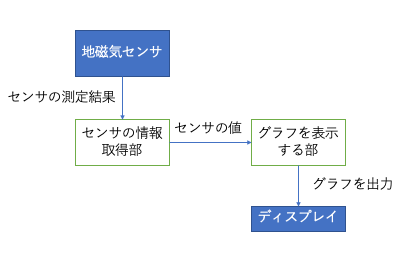
\includegraphics[scale=0.4]{機能構成図.png}
  \caption{機能構成図}
\end{figure}

 
 \subsection{開発に用いたプログラミング言語と開発環境}
 開発に使用したものを以下の表にまとめる.

 \begin{table}[h]
    \caption{開発に使用したもの}
    \centering
    \begin{tabular}{clcl}
    \hline
    OS     &  & macOS Big Sur                      &  \\ \hline
    開発環境   &  & \multicolumn{1}{l}{Android Stusio} &  \\ \hline
    使用した言語 &  & Java                               &  \\ \hline
    \end{tabular}
    \end{table}

\section{内部仕様}

\subsection{各ハードウェアが備えるソフトウェアの詳細な設計}

地磁気センサから情報を取得するために、要素数3、float型の配列をあらかじめ準備しておく。
地磁気センサの戻り値は要素数3のfloat型配列となっている。以下はその配列の中身を具体的に示した
物である。

\begin{table}[h]
  \caption{地磁気センサの戻り値}
  \centering
  \begin{tabular}{lllll}
  \hline
  \multicolumn{1}{c}{TYPE\_MAGNETIC\_FIELD} &  & SensorEvents.value{[}0{]} &  & X軸方向の地磁気強度 \\ \cline{2-5} 
                                            &  & SensorEvents.value{[}1{]} &  & Y軸方向の地磁気強度 \\ \cline{2-5} 
                                            &  & SensorEvents.value{[}2{]} &  & Z軸方向の地磁気強度 \\ \hline
  \end{tabular}
  \end{table}

\subsection{各ハードウェアが備えるソフトウェアにおける処理の流れ}
このプログラムはまず、地磁気センサから情報を取得し、取得した値をあらかじめ
準備しておいた配列へ代入、そして、配列の中身をグラフへ出力といった工程を
無限ループで回すことによって常に最新の値がグラフへ出力されるようになっている。\\
以下はフローチャートである。\\

\begin{figure}[h]
    \centering
    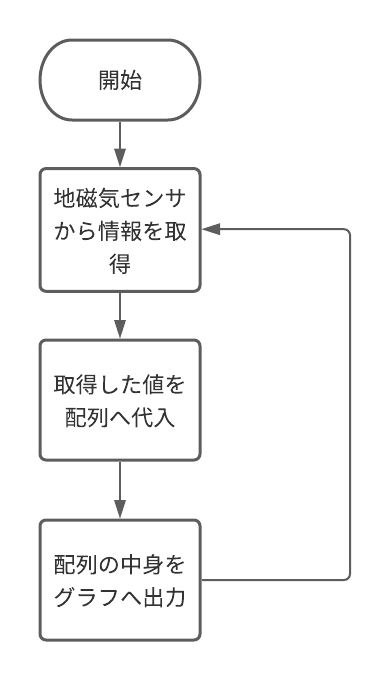
\includegraphics[scale=0.4]{flowchart.png}
    \caption{フローチャート}
\end{figure}



\section{実行例}

実行例1は適当な値をそれぞれの軸に設定した時の結果である。その後、それぞれのパラ
メータを自由に書き換えた後の結果が実行例2である。1、2より入力された値が正しく
出力されることがわかる。

\begin{figure}[h]
  \begin{minipage}[b]{0.45\linewidth}
  \begin{center}
    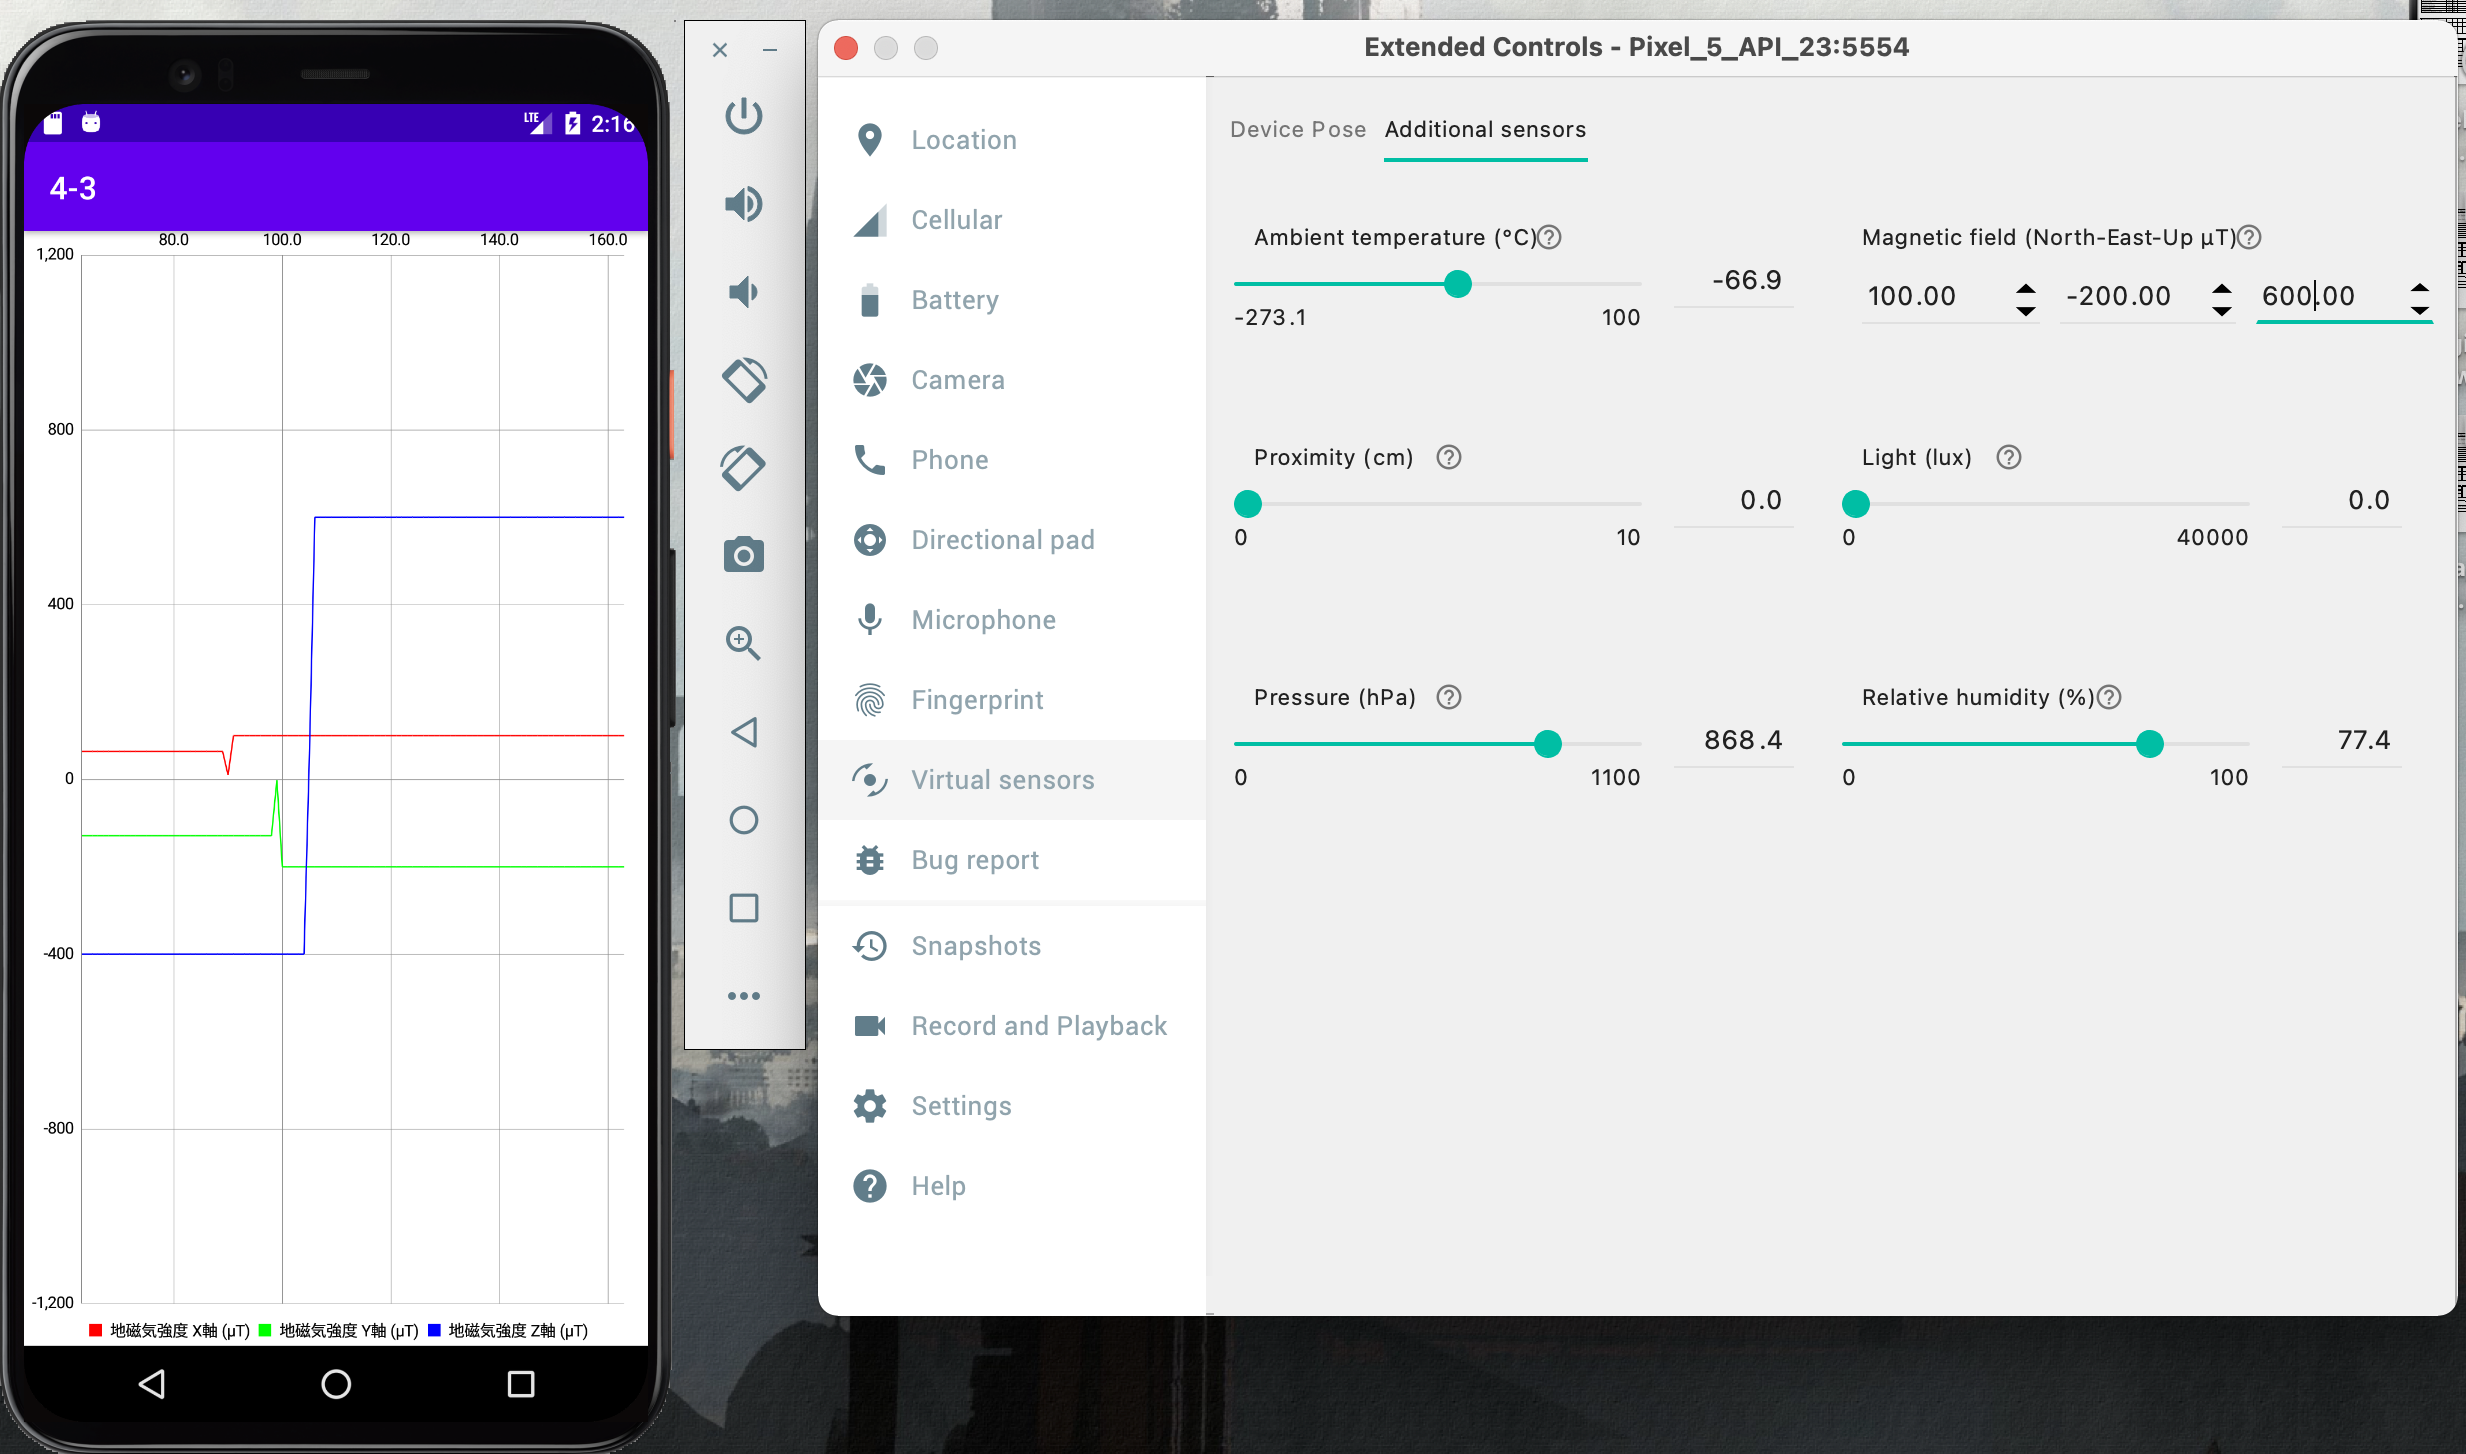
\includegraphics[keepaspectratio,scale=0.15]{pic2.png}
    \end{center}
    \caption{実行例1}
  \end{minipage}
  \begin{minipage}[b]{0.45\linewidth}
  \begin{center}
    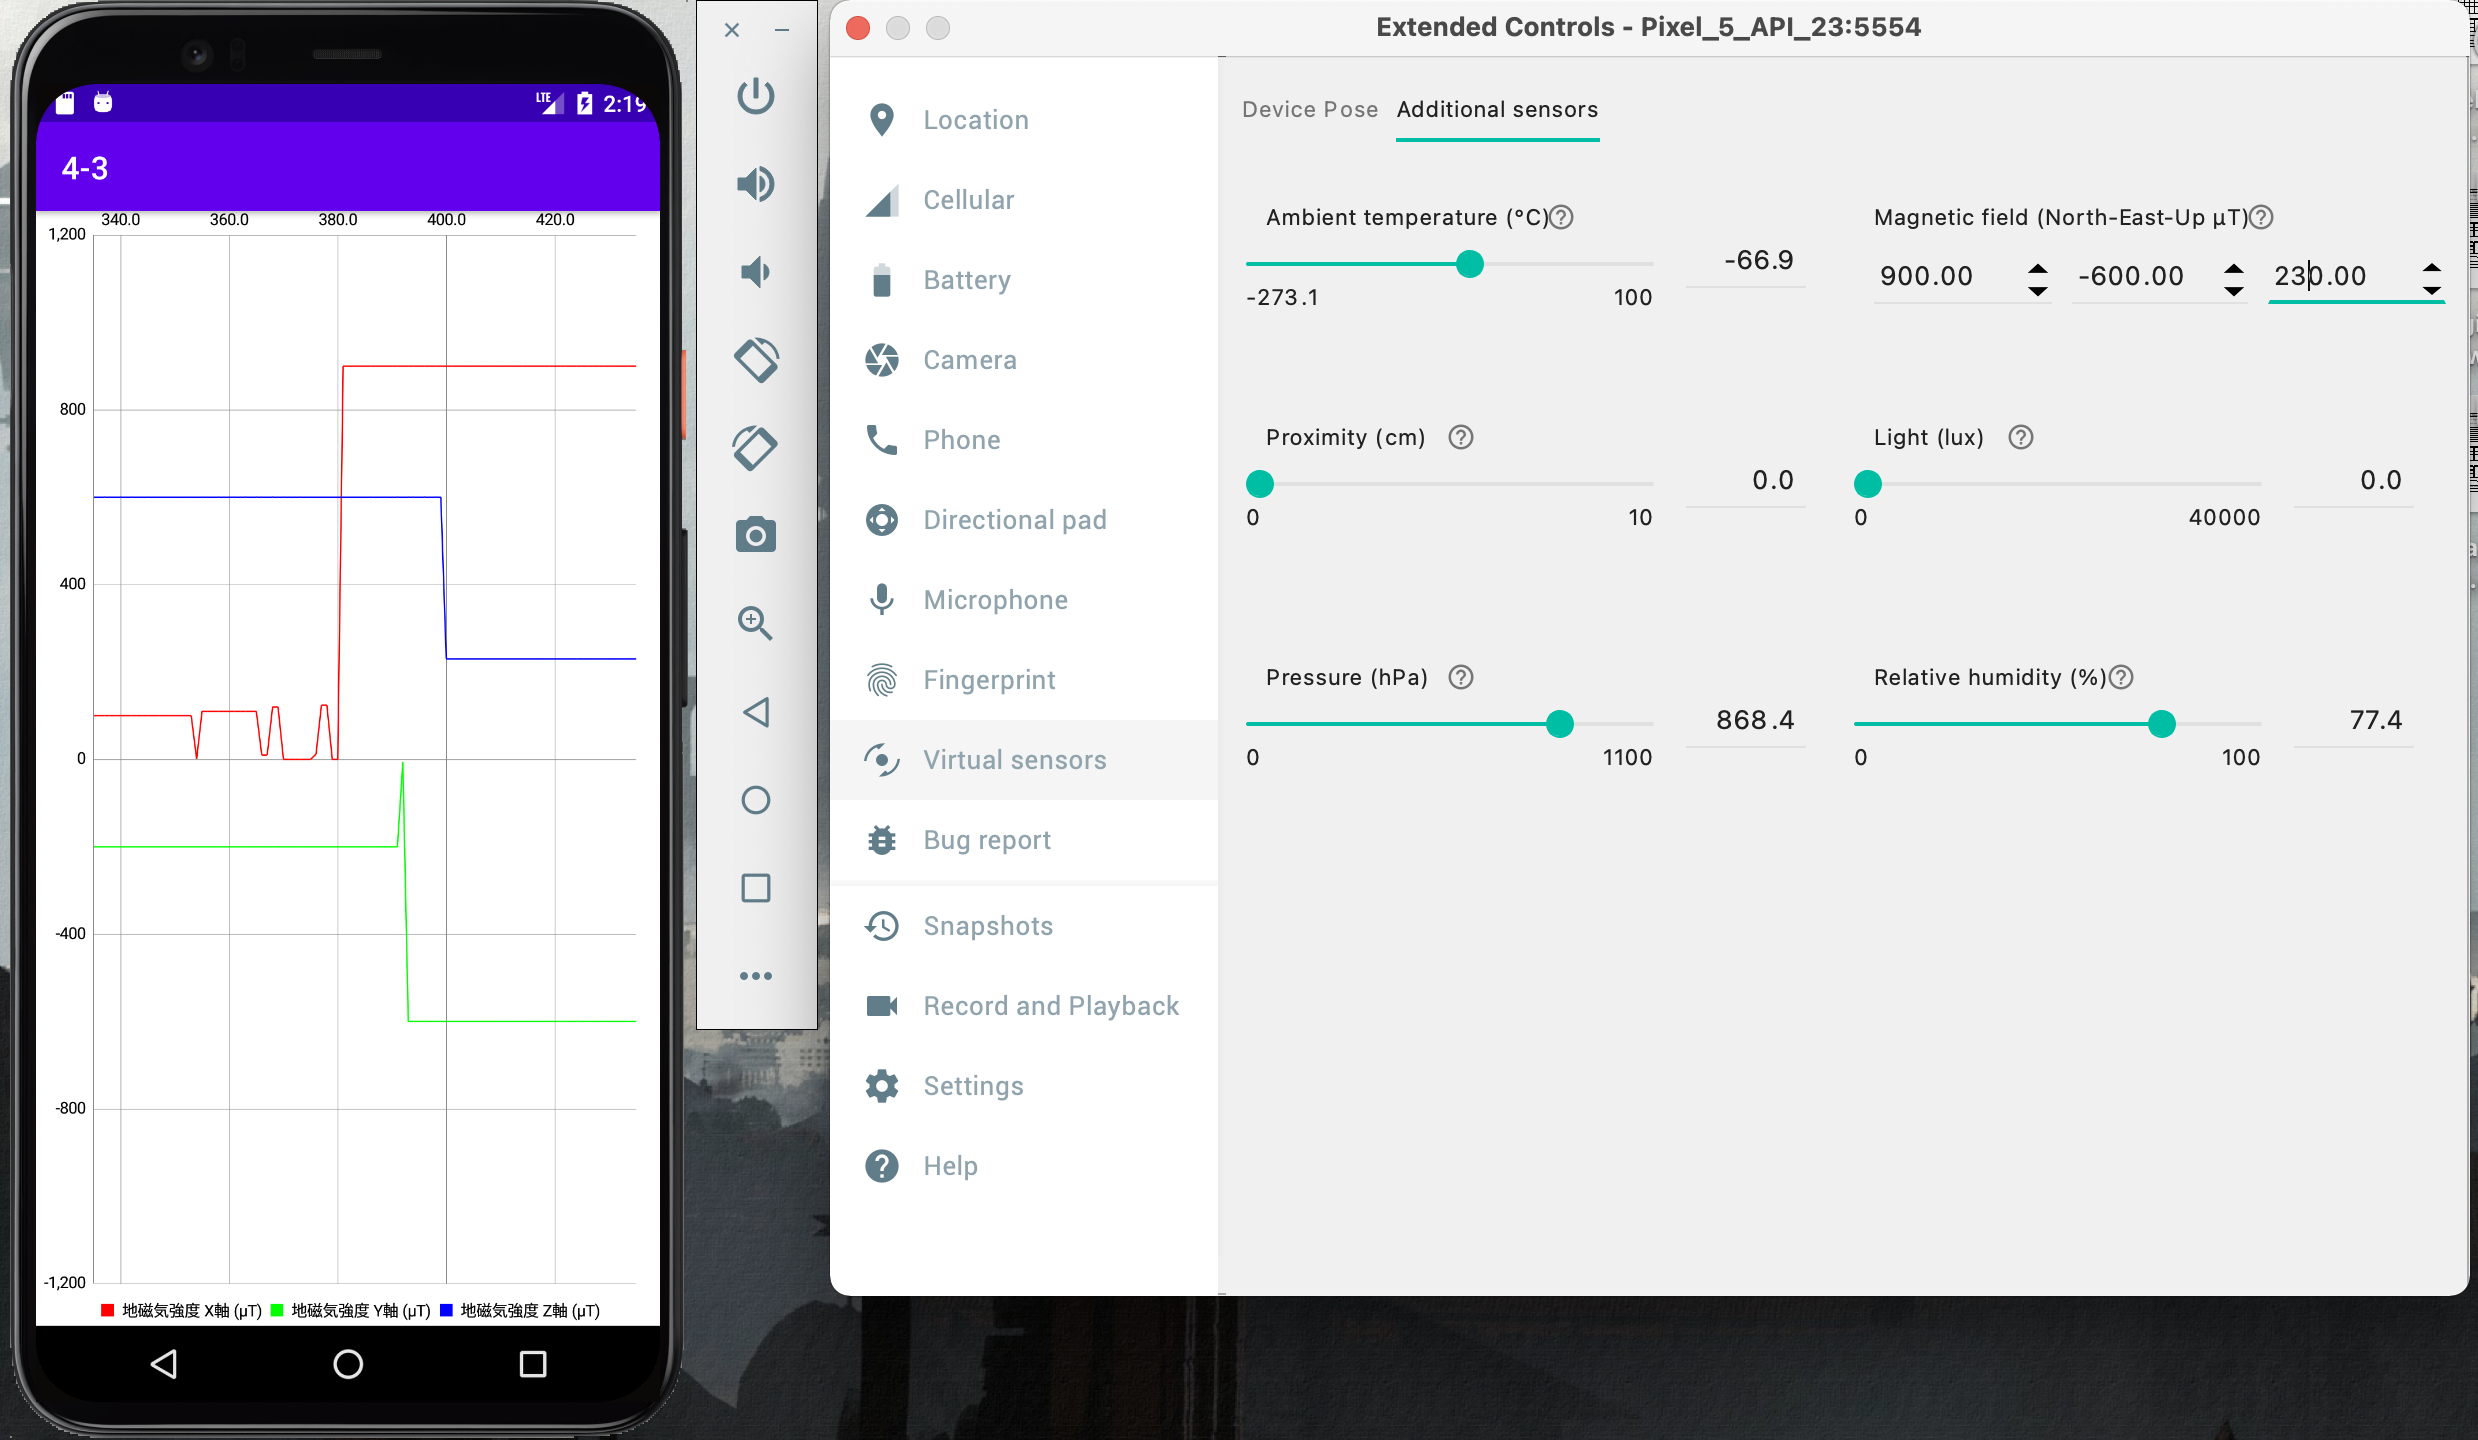
\includegraphics[keepaspectratio,scale=0.15]{pic3.png}
    \end{center}
    \caption{実行例2}
  \end{minipage}
\end{figure}


\section{ソースコード}

プログラムの説明はコード中にコメントアウトすることでおこなっている。\\
以下はソースコードである。

\lstset{
  basicstyle={\ttfamily},
  identifierstyle={\small},
  commentstyle={\smallitshape},
  keywordstyle={\small\bfseries},
  ndkeywordstyle={\small},
  stringstyle={\small\ttfamily},
  frame={tb},
  breaklines=true,
  columns=[l]{fullflexible},
  numbers=left,
  xrightmargin=0zw,
  xleftmargin=3zw,
  numberstyle={\scriptsize},
  stepnumber=1,
  numbersep=1zw,
  lineskip=-0.5ex
}

\begin{lstlisting}[caption=MainActivity.jave,label=java]
  package com.example.a4_3;

  import androidx.appcompat.app.AppCompatActivity;
  
  import android.content.Context;
  import android.hardware.Sensor;
  import android.hardware.SensorEvent;
  import android.hardware.SensorEventListener;
  import android.hardware.SensorManager;
  import android.view.WindowManager;
  import android.widget.TextView;
  
  import java.util.List;
  
  import android.os.Bundle;
  
  import android.graphics.Color;
  import android.util.Log;
  import android.view.WindowManager;
  
  import com.github.mikephil.charting.charts.LineChart;
  import com.github.mikephil.charting.components.AxisBase;
  import com.github.mikephil.charting.components.XAxis;
  import com.github.mikephil.charting.components.YAxis;
  import com.github.mikephil.charting.data.Entry;
  import com.github.mikephil.charting.data.LineData;
  import com.github.mikephil.charting.data.LineDataSet;
  import com.github.mikephil.charting.formatter.IAxisValueFormatter;
  import com.github.mikephil.charting.utils.Transformer;
  import com.github.mikephil.charting.utils.ViewPortHandler;
  
  public class MainActivity extends AppCompatActivity implements SensorEventListener {
  
      private LineChart mLineChart;
  
      // センサーマネージャを定義
      private SensorManager manager;
  
      // センサーから届いた値を格納する配列を定義
      private float[] values = new float[3];
  
      // グラフに表示するデータに関する値を定義
      private int num; // グラフにプロットするデータの数
  
      private String[] labels; // データのラベルを格納する配列
      private int[] colors; // グラフにプロットする点の色を格納する配列
      private float max, min; // グラフのY軸の最大値と最小値
  
      // 値をプロットするx座標
      private float count = 0;
  
      @Override
      protected void onResume() {
          super.onResume();
  
      // 情報を取得するセンサーの設定(今回は地磁気強度)
          List<Sensor> sensors = manager.getSensorList(Sensor.TYPE_MAGNETIC_FIELD);
          Sensor sensor = sensors.get(0);
  
      // センサーからの情報の取得を開始
          manager.registerListener(this, sensor, SensorManager.SENSOR_DELAY_UI);
      }
  
      // アプリケーション一時停止時に呼ばれるコールバック関数
      @Override
      protected void onPause() {
          super.onPause();
  
      // センサのリスナー登録解除
          manager.unregisterListener(this);
      }
  
      // センサーイベント受信時に呼ばれるコールバック関数
      public void onSensorChanged(SensorEvent event) {
          // 取得した情報が地磁気強度センサーからのものか確認
          if (event.sensor.getType() == Sensor.TYPE_MAGNETIC_FIELD) {
          // 受け取った情報を格納用の配列にコピー
              values = event.values.clone();
          }
      }
  
      // センサーの精度の変更時に呼ばれるコールバック関数(今回は何もしない)
      public void onAccuracyChanged(Sensor sensor, int accuracy) {
      }
  
      @Override
      protected void onCreate(Bundle savedInstanceState) {
          super.onCreate(savedInstanceState);
          setContentView(R.layout.activity_main);
  
          manager = (SensorManager) getSystemService(Context.SENSOR_SERVICE);
  
          // アプリ実行中はスリープしない
          getWindow().addFlags(WindowManager.LayoutParams.FLAG_KEEP_SCREEN_ON);
  
          // グラフに表示するデータに関連する値を初期化
          num = 3;
          values = new float[num];
          labels = new String[num];
          colors = new int[num];
  
          labels[0] = "地磁気強度 X軸 (μT)";
          labels[1] = "地磁気強度 Y軸 (μT)";
          labels[2] = "地磁気強度 Z軸 (μT)";
  
          colors[0] = Color.rgb(0xFF, 0x00, 0x00); // 赤
          colors[1] = Color.rgb(0x00, 0xFF, 0x00); // 緑
          colors[2] = Color.rgb(0x00, 0x00, 0xFF); // 青
  
          max = 1200;
          min = -1200;
  
          // グラフViewを初期化する
          initChart();
  
          // 一定間隔でグラフをアップデートする
          new Thread(new Runnable() {
              @Override
              public void run() {
                  while (true) {
                      updateGraph();
                      try {
                          Thread.sleep(500);
                      } catch (Exception e) {
                          Log.e("Test", "例外出力", e);
                      }
                  }
              }
          }).start();
      }
  
      /**
       * グラフViewの初期化
       **/
  
      private void initChart() {
          // 線グラフView
          mLineChart = (LineChart) findViewById(R.id.chart_DynamicMultiLineGraph);
  
          // グラフ説明テキストを表示するか
          mLineChart.getDescription().setEnabled(true);
          // グラフ説明テキストのテキスト設定
          mLineChart.getDescription().setText("Line Chart of Sensor Data");
          // グラフ説明テキストの文字色設定
          mLineChart.getDescription().setTextColor(Color.BLACK);
          // グラフ説明テキストの文字サイズ設定
          mLineChart.getDescription().setTextSize(10f);
          // グラフ説明テキストの表示位置設定
          mLineChart.getDescription().setPosition(0, 0);
  
          // グラフへのタッチジェスチャーを有効にするか
          mLineChart.setTouchEnabled(true);
  
          // グラフのスケーリングを有効にするか
          mLineChart.setScaleEnabled(true);
  
          // グラフのドラッギングを有効にするか
          mLineChart.setDragEnabled(true);
  
          // グラフのピンチ/ズームを有効にするか
          mLineChart.setPinchZoom(true);
  
          // グラフの背景色設定
          mLineChart.setBackgroundColor(Color.WHITE);
  
          // 空のデータをセットする
          mLineChart.setData(new LineData());
  
          // Y軸(左)の設定
          // Y軸(左)の取得
          YAxis leftYAxis = mLineChart.getAxisLeft();
          // Y軸(左)の最大値設定
          leftYAxis.setAxisMaximum(max);
          // Y軸(左)の最小値設定
          leftYAxis.setAxisMinimum(min);
  
          // Y軸(右)の設定
          // Y軸(右)は表示しない
          mLineChart.getAxisRight().setEnabled(false);
  
          // X軸の設定
          XAxis xAxis = mLineChart.getXAxis();
          // X軸の値表示設定
          xAxis.setValueFormatter(new IAxisValueFormatter() {
              @Override
              public String getFormattedValue(float value, AxisBase axis) {
                  if (value >= 10) {
                      // データ20個ごとに目盛りに文字を表示
                      if (((int) value % 20) == 0) {
                          return Float.toString(value);
                      }
                  }
                  // nullを返すと落ちるので、値を書かない場合は空文字を返す
                  return "";
              }
          });
      }
  
      private void updateGraph() {
          // 線の情報を取得
          LineData lineData = mLineChart.getData();
          if (lineData == null) {
              return;
          }
  
          LineDataSet[] lineDataSet = new LineDataSet[num];
  
          for (int i = 0; i < num; i++) {
              // i番目の線を取得
              lineDataSet[i] = (LineDataSet) lineData.getDataSetByIndex(i);
              // i番目の線が初期化されていない場合は初期化する
              if (lineDataSet[i] == null) {
                  // LineDataSetオブジェクト生成
                  lineDataSet[i] = new LineDataSet(null, labels[i]);
                  // 線の色設定
                  lineDataSet[i].setColor(colors[i]);
                  // 線にプロット値の点を描画しない
                  lineDataSet[i].setDrawCircles(false);
                  // 線にプロット値の値テキストを描画しない
                  lineDataSet[i].setDrawValues(false);
                  // 線を追加
                  lineData.addDataSet(lineDataSet[i]);
              }
              // i番目の線に値を追加
              lineData.addEntry(new Entry(count, values[i]), i);
          }
  
          // 値更新通知
          mLineChart.notifyDataSetChanged();
  
          // X軸に表示する最大のEntryの数を指定
          mLineChart.setVisibleXRangeMaximum(100);
  
          // オシロスコープのように古いデータを左に寄せていくように表示位置をずらす
          mLineChart.moveViewTo(count, getVisibleYCenterValue(mLineChart), YAxis.AxisDependency.LEFT);
  
          count++;
      }
  
      private float getVisibleYCenterValue(LineChart lineChart) {
          Transformer transformer = lineChart.getTransformer(YAxis.AxisDependency.LEFT);
          ViewPortHandler viewPortHandler = lineChart.getViewPortHandler();
  
          float highestVisibleY = (float) transformer.getValuesByTouchPoint(viewPortHandler.contentLeft(),
                  viewPortHandler.contentTop()).y;
          float highestY = Math.min(lineChart.getAxisLeft().mAxisMaximum, highestVisibleY);
  
          float lowestVisibleY = (float) transformer.getValuesByTouchPoint(viewPortHandler.contentLeft(),
                  viewPortHandler.contentBottom()).y;
          float lowestY = Math.max(lineChart.getAxisLeft().mAxisMinimum, lowestVisibleY);
  
          return highestY - (Math.abs(highestY - lowestY) / 2);
      }
  }
  
\end{lstlisting}


\end{document}